\scanpage{53}
\mspage{\handwritten{21}}
% archive sheet number: 52

$G=\underset{\handwritten{\longleftarrow}}{\lim}G_i$ (EGA IV 8.2 3). \deleted{Le fait que} les morphismes de transition sont fidèle-\linebreak \makebox[0pt][l]{\hspace{.7em}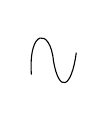
\begin{tikzpicture}[x=1cm,y=1cm,baseline=0pt]\draw (-.22,-.16) .. controls (-.26,.43) and (.02,.43) .. (.06,.02) .. controls (.13,-.4) and (.29,-.34) .. (.35,.12);\end{tikzpicture}}mnet plats d'après le lemme suivant :


\uline{Lemme \handwritten{11.14}.- Soient $k$ un corps, $G$ et $H$ deux $k$-groupes affines de type fini, $u:G\handwritten{\longrightarrow}H$} un \uline{morphisme de $k$-groupes, et $u^{\unsure{o|0|\circ}}:B\handwritten{\longrightarrow}A$ l'homomorphisme de $k$-algèbres correspondant .} Pour que \uline{$u$ soit fidèlement plat, il faut et il suffit que $u^{\unsure{o|0|\circ}}$ soit injectif.}

la condition est évidemment nécessaire (EGA IV 2.2.3 et $\unsure{0|O}_{\mathrm{IV}}$ 6.6.1). Montrons qu'elle est suffisante. Posons $K=\operatorname{Ker}u$. Alors $G/K$ est un $k$-groupe\inserted{\makebox[0pt][l]{\hspace{1.05cm}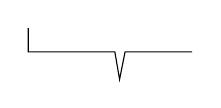
\begin{tikzpicture}[x=1cm,y=1cm,baseline=0pt]\draw (-1.05,.1)--(-1.05,-.2)--(.05,-.2)--(.11,-.55)--(.18,-.2)--(1.03,-.2);\end{tikzpicture}}de type fini} (\deleted{Exp.} $\mathrm{VI}_A$ 5.2), et $u$ se factorise en \begin{tikzcd}[ampersand replacement=\&,cramped,column sep=small]G\arrow[r,"{\inserted{p}}","{\deleted{\unsure{p}}}" description]\&G/K\arrow[r,"v"]\&H\end{tikzcd}, où $p$ est fidèlement plat (\deleted{Exp.} $\mathrm{VI}_A$ 3.2) et où $v$ est un monomorphisme de $k$-groupes de type fini, donc une immersion fermée (1.4.2). Puisque $H$ est un schéma affine, et que $v$ est une immersion fermée, $G/K$ est un schéma affine (EGA I 4.2.3), et, si on note $C$ l'algèbre de $G/K$, l'homomorphisme $v^{\unsure{o|0|\circ}}:B\handwritten{\longrightarrow}C$ est surjectif (loc. cit.) Or, puisque $u^{\unsure{o|0|\circ}}$ est injectif, et que $u^{\unsure{o|0|\circ}}=p^{\unsure{o|0|\circ}}\mathbin{o}v^{\unsure{o|0|\circ}}$, $v^{\unsure{o|0|\circ}}$ est aussi injectif : c'est un isomorphisme, donc $v$ est un isomorphisme, et, puisque $p$ est fidèlement plat, il en est de même de $u$.

\uline{Définitions \handwritten{11.15}}.- Etant donné un corps $k$, un $k$-espace vectoriel $V$, un $k$-groupe $G$ opérant sur $V$, et un vecteur $v\in V$, on dit que $v$ est \uline{semi-invariant} sous $G$ si le sous-espace vectoriel $\handwritten{k.v}$ \deleted{soit}\handwritten{est} stable sous $G$.
\margin{\handwritten{\makebox[0pt][l]{\hspace{.45cm}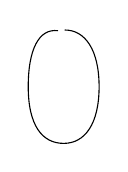
\begin{tikzpicture}[x=0.45cm,y=0.45cm,baseline=0pt]\draw (-.16,1.58) .. controls (-.7,1.65) and (-1,1.05) .. (-1,0) .. controls (-1,-1.1) and (-.6,-1.6) .. (0,-1.6) .. controls (.6,-1.6) and (1,-1.05) .. (1,0) .. controls (1,1.05) and (.6,1.6) .. (.03,1.6);\end{tikzpicture}}\shortstack{à la\\ligne}}}
\figure{\handwritten{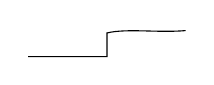
\begin{tikzpicture}[x=0.5cm,y=0.3cm]\draw (0,0) -- (2,0) -- (2,1) .. controls (2.5,1.2) and (3.3,1) .. (4,1.1);\end{tikzpicture}}}
Notons $A$ l'algèbre de $G$, et $\handwritten{\rho}:V\handwritten{\longrightarrow}A\handwritten{\otimes}_k V$ l'application linéaire qui dé-\linebreak finit l'opération de $G$ sur $V$. Dire que $v$ est semi-invariant sous $G$ revient à dire \deleted{que, pour} qu'il existe $\handwritten{\lambda}\in A$ tel que, pour tout $w\in kv$, $\handwritten{\rho}(w)=\handwritten{\lambda\otimes}w$. Lorsque $v\handwritten{\neq}0$, l'élément $\handwritten{\lambda\in}A$ est bien déterminé par cette relation, on l'appellera \deleted{\uline{invariant}}\inserted{\handwritten{\uline{poids}}} de l'élément semi-invariant $\handwritten{v}$.

\deleted{D'autre part, $v$ s'interprête comme un élément du bidual de $V$, donc comme une section de $\handwritten{\mathbb{V}}(V)$; notons $\handwritten{\varphi}:G\handwritten{\times\mathbb{V}}(V)\handwritten{\longrightarrow\mathbb{V}}(V)$ le morphisme définissant l'opération de $G$ sur $V$.} Dire que $v$ est semi-invariant \deleted{revient à dire qu'il existe $\unsure{g|\lambda|?}\in k$} d'invariant $\handwritten{\lambda}$ revient à dire que $\handwritten{\varphi}(g,v)=\handwritten{\unsure{\deleted{\chi}\inserted{\lambda}|\lambda}}(g)v$ pour tout $g\in G(k)$, où $\deleted{\handwritten{\unsure{\varphi|\chi}:\unsure{k|G}\longrightarrow\unsure{\mathbb{G}_k|\underline{G}_{m,k}}}}\inserted{\handwritten{\unsure{\deleted{\chi}\inserted{\lambda}|\lambda}:G\longrightarrow\underline{G}_{m,k}}}$ est le morphisme défini par $\handwritten{\lambda}$. On voit donc que $\handwritten{\lambda}$ \deleted{correspond à}\inserted{\handwritten{est}} un caractère \deleted{\handwritten{$\unsure{\chi|\lambda}$}} de $G$, appelé \uline{caractère associé} à l'élément semi-inva-\linebreak riant $v$. \deleted{Enfin nous appellerons \uline{poids} de l'élément semi-invariant $v$ le poids du caractère $\handwritten{\chi}$ associé à $v$.}
\margin{\handwritten{!}}
